\documentclass{beamer}
\usepackage[utf8]{inputenc}
\usepackage{graphicx, epsfig}
\usepackage{amsmath,mathrsfs,amsfonts,amssymb}
\usepackage{floatflt}
\usepackage{epic,ecltree}
\usepackage{mathtext}
\usepackage{fancybox}
\usepackage{fancyhdr}
\usepackage{multirow}
\usepackage{enumerate}
\usepackage{epstopdf}
\usepackage{multicol}
\usepackage{algorithm}
\usepackage[noend]{algorithmic}
\usepackage{tikz}
\usepackage{blindtext}
\usetheme{default}%{Singapore}%{Warsaw}%{Warsaw}%{Darmstadt}
\usecolortheme{default}

\setbeamerfont{title}{size=\Huge}
\setbeamertemplate{footline}[page number]{}

\setbeamertemplate{section in toc}[sections numbered]


\makeatletter
\newcommand\HUGE{\@setfontsize\Huge{35}{40}}
\makeatother    

\setbeamerfont{title}{size=\HUGE}
\beamertemplatenavigationsymbolsempty

% latin bold lower
\newcommand{\ba}{\mathbf{a}} 
\newcommand{\bc}{\mathbf{c}} 
\newcommand{\be}{\mathbf{e}} 
\newcommand{\bh}{\mathbf{h}} 
\newcommand{\bp}{\mathbf{p}} 
\newcommand{\bt}{\mathbf{t}} 
\newcommand{\bs}{\mathbf{s}} 
\newcommand{\bu}{\mathbf{u}} 
\newcommand{\bv}{\mathbf{v}} 
\newcommand{\bw}{\mathbf{w}} 
\newcommand{\bx}{\mathbf{x}} 
\newcommand{\by}{\mathbf{y}} 
\newcommand{\bz}{\mathbf{z}} 

% latin bold upper
\newcommand{\bA}{\mathbf{A}} 
\newcommand{\bB}{\mathbf{B}} 
\newcommand{\bC}{\mathbf{C}} 
\newcommand{\bI}{\mathbf{I}} 
\newcommand{\bL}{\mathbf{L}} 
\newcommand{\bM}{\mathbf{M}} 
\newcommand{\bQ}{\mathbf{Q}} 
\newcommand{\bT}{\mathbf{T}} 
\newcommand{\bU}{\mathbf{U}} 
\newcommand{\bV}{\mathbf{V}} 
\newcommand{\bW}{\mathbf{W}} 
\newcommand{\bX}{\mathbf{X}} 
\newcommand{\bY}{\mathbf{Y}} 
\newcommand{\bZ}{\mathbf{Z}} 

% latin cal upper
\newcommand{\cG}{\mathcal{G}} 
\newcommand{\cL}{\mathcal{L}} 
\newcommand{\cN}{\mathcal{N}} 
\newcommand{\cS}{\mathcal{S}} 
\newcommand{\cT}{\mathcal{T}} 
\newcommand{\cW}{\mathcal{W}} 
\newcommand{\cX}{\mathcal{X}} 
\newcommand{\cZ}{\mathcal{Z}} 

% latin bb upper
\newcommand{\bbE}{\mathbb{E}} 
\newcommand{\bbI}{\mathbb{I}} 
\newcommand{\bbP}{\mathbb{P}} 
\newcommand{\bbR}{\mathbb{R}} 

% greek bold lower
\newcommand{\bepsilon}{\boldsymbol{\epsilon}} 
\newcommand{\btheta}{\boldsymbol{\theta}} 
\newcommand{\blambda}{\boldsymbol{\lambda}} 
\newcommand{\bpi}{\boldsymbol{\pi}} 
\newcommand{\bmu}{\boldsymbol{\mu}} 
\newcommand{\bsigma}{\boldsymbol{\sigma}} 
\newcommand{\bphi}{\boldsymbol{\phi}} 

% greek bold upper
\newcommand{\bSigma}{\boldsymbol{\Sigma}} 

\DeclareMathOperator*{\argmin}{arg\,min}
\DeclareMathOperator*{\argmax}{arg\,max}

\newcommand{\createdgmtitle}[1]{\title[\hbox to 56mm{Deep Generative Models  \hfill\insertframenumber\,/\,\inserttotalframenumber}]
	{Deep Generative Models \\ {\Huge Lecture #1}}
	\author{Roman Isachenko}
	\institute{
\includegraphics[width=0.5cm]{../utils/ozonmasterslogo} \large{Ozon Masters}}
	\date{Spring, 2022}
}

\newcommand\myfootnote[1]{%
  \tikz[remember picture,overlay]
  \draw (current page.south west) +(1in + \oddsidemargin,0.5em)
  node[anchor=south west,inner sep=0pt]{\parbox{\textwidth}{%
      \rlap{\rule{10em}{0.4pt}}\raggedright\scriptsize \textit{#1}}};}

\newcommand\myfootnotewithlink[2]{%
  \tikz[remember picture,overlay]
  \draw (current page.south west) +(1in + \oddsidemargin,0.5em)
  node[anchor=south west,inner sep=0pt]{\parbox{\textwidth}{%
      \rlap{\rule{10em}{0.4pt}}\raggedright\scriptsize\href{#1}{\textit{#2}}}};}
      
\AtBeginSection[]
{
	\begin{frame}{Outline}
		\tableofcontents[currentsection,subsectionstyle=hide]
	\end{frame}
}
\AtBeginSubsection[]{
	\begin{frame}{Outline}
		\tableofcontents[currentsection,currentsubsection]
	\end{frame}
}
\createdgmtitle{7}
%--------------------------------------------------------------------------------
\begin{document}
%--------------------------------------------------------------------------------
\begin{frame}[noframenumbering,plain]
%\thispagestyle{empty}
\titlepage
\end{frame}
%=======
\begin{frame}{Recap of previous lecture}
	\begin{block}{Gaussian autoregressive flow (MAF)}
		\vspace{-0.8cm}
		\begin{align*}
			\bx &= g(\bz, \btheta) \quad \Rightarrow \quad x_i = \sigma_i (\bx_{1:i-1}) \cdot z_i + \mu_i(\bx_{1:i-1}). \\
			\bz &= f(\bx, \btheta) \quad \Rightarrow \quad z_i = \left(x_i - \mu_i(\bx_{1:i-1}) \right) \cdot \frac{1}{ \sigma_i (\bx_{1:i-1})}.
		\end{align*}
		Generation function $g(\bz, \btheta)$ is \textbf{sequential}. Inference function $f(\bx, \btheta)$ is \textbf{not sequential}.
	\end{block}
	\begin{block}{Inverse autoregressive flow (IAF)}
		\vspace{-0.5cm}
		\begin{align*}
			\bx &= g(\bz, \btheta) \quad \Rightarrow \quad x_i = \tilde{\sigma}_i (\bz_{1:i-1}) \cdot z_i + \tilde{\mu}_i(\bz_{1:i-1}) \\
			\bz &= f(\bx, \btheta) \quad \Rightarrow \quad z_i = \left( x_i - \tilde{\mu}_i(\bz_{1:i-1})\right) \cdot \frac{1}{\tilde{\sigma}_i (\bz_{1:i-1}) }.
		\end{align*}
		\vspace{-0.3cm}
	\end{block}
		
	\myfootnote{
	\href{https://arxiv.org/abs/1705.07057}{Papamakarios G., Pavlakou T., Murray I. Masked Autoregressive Flow for Density Estimation, 2017} \\
	\href{https://arxiv.org/abs/1606.04934}{Kingma D. P. et al. Improving Variational Inference with Inverse Autoregressive Flow, 2016} } 
\end{frame}
%=======
\begin{frame}{Recap of previous lecture}
	\begin{block}{Autoregressive flows}
		\begin{figure}
			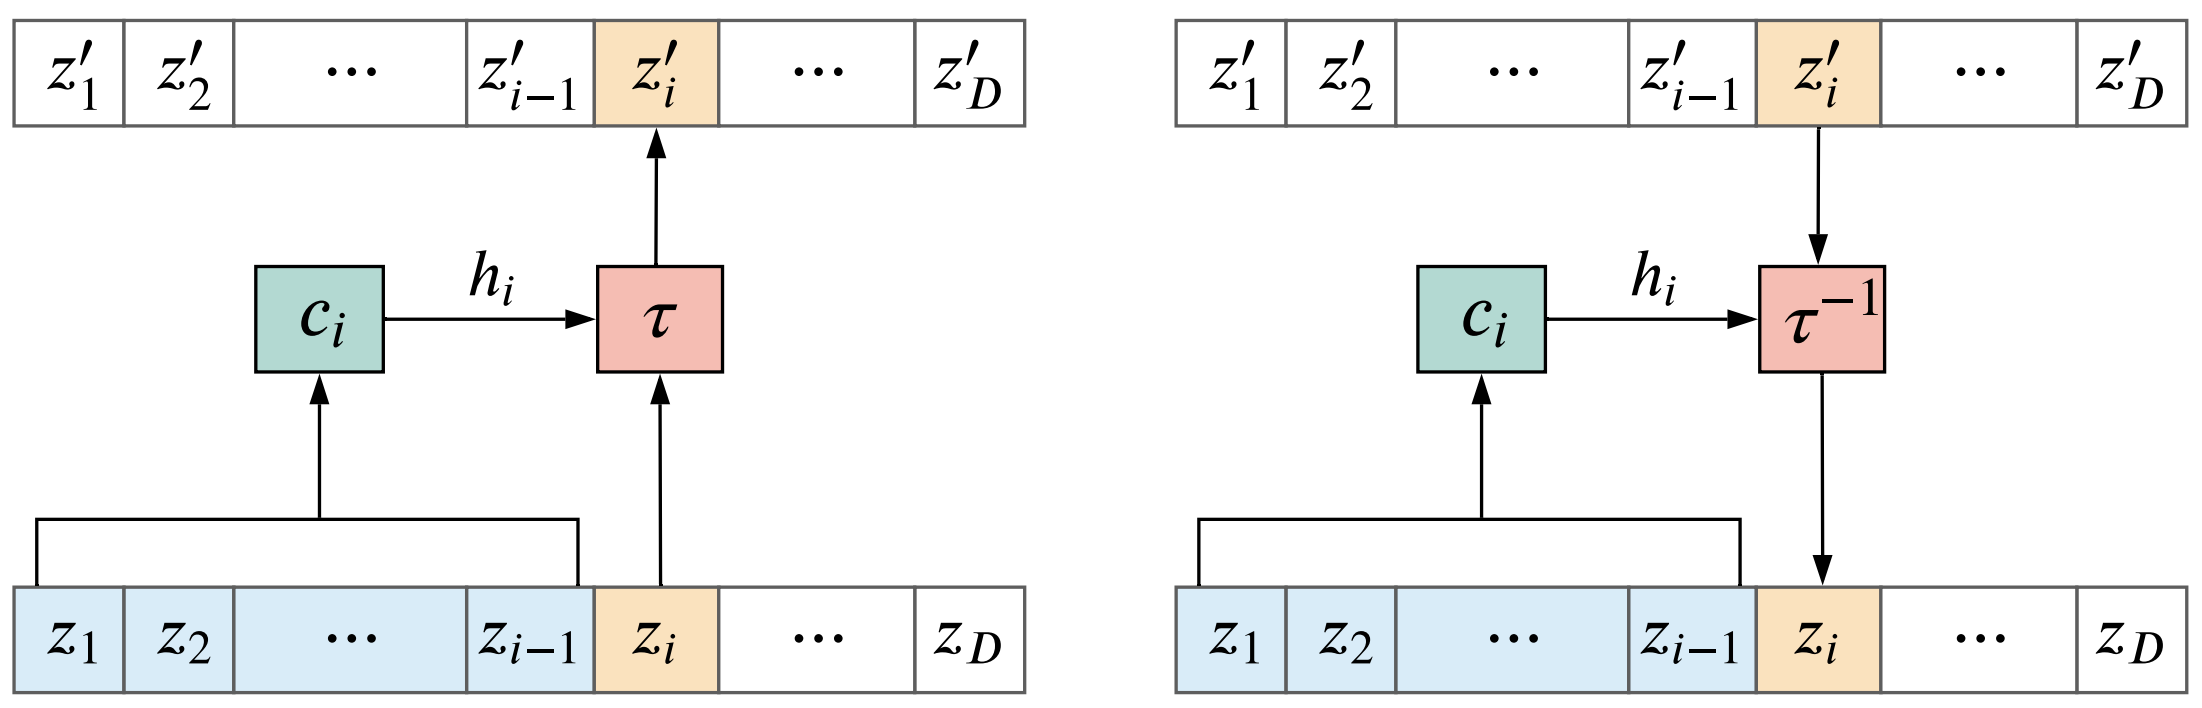
\includegraphics[width=0.9\linewidth]{figs/autoregressive_flow}
		\end{figure}
	\end{block}
	\begin{block}{RealNVP: Affine coupling law}
		\vspace{-0.7cm}
		\[
			\begin{cases} \bz_{1:d} = \bx_{1:d}; \\ \bz_{d:m} = \tau (\bx_{d:m}, c(\bx_{1:d}));\end{cases} 
			\quad \Leftrightarrow \quad 
			\begin{cases} \bx_{1:d} = \bz_{1:d}; \\ \bx_{d:m} = \tau^{-1} (\bz_{d:m}, c(\bz_{1:d})).\end{cases}
		\]
	\end{block}
	\myfootnote{
	\href{https://arxiv.org/abs/1410.8516}{Dinh L., Krueger D., Bengio Y. NICE: Non-linear Independent Components Estimation, 2014} \\
	\href{https://arxiv.org/abs/1605.08803}{Dinh L., Sohl-Dickstein J., Bengio S. Density estimation using Real NVP, 2016}}
\end{frame}
%=======
\begin{frame}{Outline}
	\tableofcontents
\end{frame}
\AtBeginSection[ ]
{
	\begin{frame}{Outline}
		\tableofcontents[currentsection]
	\end{frame}
}
%=======
\begin{frame}{Likelihood-based models}
\begin{block}{Exact likelihood evaluation}
	\begin{itemize}
		\item Autoregressive models (WaveNet, PixelCNN, PixelCNN++);
		\item Flow models (RealNVP, IAF, Glow).
	\end{itemize}
\end{block}
\begin{block}{Approximate likelihood evaluation}
	\begin{itemize}
		\item Latent variable models (VAE).
	\end{itemize}
\end{block}
What are the pros and cons of each of them? \\
\vspace{0.2cm}
\end{frame}
%=======
\begin{frame}{VAE limitations}
	\begin{itemize}
		\item Poor generative distribution (decoder)
		\[
			p(\bx | \bz, \btheta) = \mathcal{N}(\bx| \bmu_{\btheta}(\bz), \bsigma^2_{\btheta}(\bz)) \quad \text{or } = \text{Softmax}(\bpi_{\btheta}(\bz)).
		\]
		\item Loose lower bound
		\[
			\log p(\bx | \btheta) - \mathcal{L}(q, \btheta) = (?).
		\]
		\item \textbf{Poor prior distribution}
		\[
			p(\bz) = \mathcal{N}(0, \mathbf{I}).
		\]
		\item Poor variational posterior distribution (encoder)
		\[
			q(\bz | \bx, \bphi) = \mathcal{N}(\bz| \bmu_{\bphi}(\bx), \bsigma^2_{\bphi}(\bx)).
		\]
	\end{itemize}
\end{frame}
%=======
\begin{frame}{ELBO interpretations}
	\[
		\log p(\bx | \btheta) = \cL (\bphi, \btheta) + KL(q(\bz | \bx, \bphi) || p(\bz | \bx, \btheta)) \geq  \cL (\bphi, \btheta).
	\]
	\[
		\cL (\bphi, \btheta) = \int q(\bz | \bx, \bphi) \log \frac{p(\bx, \bz | \btheta)}{q(\bz | \bx, \bphi)} d \bz.
	\]
	\begin{itemize}
	    \item Evidence minus posterior KL
	    \[
	        \mathcal{L}(\bphi, \btheta) = \log p(\bx | \btheta) - KL(q(\bz | \bx, \bphi) || p(\bz | \bx, \btheta)).
	    \]
	    \item Average reconstruction loss with regularizer (prior KL)
	    \begin{align*}
	        \mathcal{L}(\bphi, \btheta) &= \mathbb{E}_{q(\bz | \bx, \bphi)} \left[ \log p(\bx | \bz, \btheta) + \log p(\bz) - \log q(\bz | \bx, \bphi) \right] \\
	        &= \mathbb{E}_{q(\bz | \bx, \bphi)} \log p(\bx | \bz, \btheta) - KL(q(\bz | \bx, \bphi) || p(\bz)).
	    \end{align*}
	\end{itemize}
\end{frame}
%=======
\begin{frame}{ELBO surgery}
	\vspace{-0.3cm}
	\[
	    \frac{1}{n} \sum_{i=1}^n \mathcal{L}_i(q, \btheta) = \frac{1}{n} \sum_{i=1}^n \left[ \mathbb{E}_{q(\bz | \bx_i)} \log p(\bx_i | \bz, \btheta) - KL(q(\bz | \bx_i) || p(\bz)) \right].
	\]
	\vspace{-0.3cm}
	\begin{block}{Theorem}
		\[
		    \frac{1}{n} \sum_{i=1}^n KL(q(\bz | \bx_i) || p(\bz)) = KL(q_{\text{agg}}(\bz) || p(\bz)) + \bbI_{q} [\bx, \bz],
		\]
		\begin{itemize}
			\item $q_{\text{agg}}(\bz) = \frac{1}{n} \sum_{i=1}^n q(\bz | \bx_i)$ -- \textbf{aggregated} posterior distribution.
			\item $\bbI_{q} [\bx, \bz]$ -- mutual information between $\bx$ and $\bz$ under empirical data distribution and distribution $q(\bz | \bx)$.
			\item First term pushes $q_{\text{agg}}(\bz)$ towards the prior $p(\bz)$.
			\item Second term reduces the amount of	information about $\bx$ stored in $\bz$. 
		\end{itemize}
	\end{block}
	\myfootnotewithlink{http://approximateinference.org/accepted/HoffmanJohnson2016.pdf}{Hoffman M. D., Johnson M. J. ELBO surgery: yet another way to carve up the variational evidence lower bound, 2016}
\end{frame}
%=======
\begin{frame}{ELBO surgery}
	\begin{block}{Theorem}
		\vspace{-0.3cm}
		\[
		    \frac{1}{n} \sum_{i=1}^n KL(q(\bz | \bx_i) || p(\bz)) = KL(q_{\text{agg}}(\bz) || p(\bz)) + \bbI_q [\bx, \bz].
		\]
		\vspace{-0.4cm}
	\end{block}
	\begin{block}{Proof}
		\vspace{-0.5cm}
		{\footnotesize
		\begin{multline*}
		    \frac{1}{n} \sum_{i=1}^n KL(q(\bz | \bx_i) || p(\bz)) = \frac{1}{n} \sum_{i=1}^n \int q(\bz | \bx_i) \log \frac{q(\bz | \bx_i)}{p(\bz)} d \bz = \\
		    = \frac{1}{n} \sum_{i=1}^n \int q(\bz | \bx_i) \log \frac{q_{\text{agg}}(\bz) q(\bz | \bx_i)}{p(\bz)q_{\text{agg}}(\bz)} d \bz 
		    = \int \frac{1}{n} \sum_{i=1}^n  q(\bz | \bx_i) \log \frac{q_{\text{agg}}(\bz)}{p(\bz)} d \bz + \\ 
		    + \frac{1}{n}\sum_{i=1}^n \int q(\bz | \bx_i) \log \frac{q(\bz | \bx_i)}{q_{\text{agg}}(\bz)} d \bz = 
		     KL (q_{\text{agg}}(\bz) || p(\bz)) + \frac{1}{n}\sum_{i=1}^n KL(q(\bz | \bx_i) || q_{\text{agg}}(\bz))
		\end{multline*}
		}
		Without proof:
		\vspace{-0.4cm}
		\[
			\bbI_{q} [\bx, \bz] = \frac{1}{n}\sum_{i=1}^n KL(q(\bz | \bx_i) || q_{\text{agg}}(\bz)) \in [0, \log n].
		\]
	\end{block}

	\myfootnotewithlink{http://approximateinference.org/accepted/HoffmanJohnson2016.pdf}{Hoffman M. D., Johnson M. J. ELBO surgery: yet another way to carve up the variational evidence lower bound, 2016}
\end{frame}
%=======
\begin{frame}{ELBO surgery}
	\begin{block}{ELBO revisiting}
		\vspace{-0.7cm}
		\begin{multline*}
		    \frac{1}{n}\sum_{i=1}^n \cL_i(q, \btheta) = \frac{1}{n} \sum_{i=1}^n \left[ \mathbb{E}_{q(\bz | \bx_i)} \log p(\bx_i | \bz, \btheta) - KL(q(\bz | \bx_i) || p(\bz)) \right] = \\
		    = \underbrace{\frac{1}{n} \sum_{i=1}^n \mathbb{E}_{q(\bz | \bx_i)} \log p(\bx_i | \bz, \btheta)}_{\text{Reconstruction loss}} - \underbrace{\vphantom{ \sum_{i=1}^n} \bbI_q [\bx, \bz]}_{\text{MI}} - \underbrace{\vphantom{ \sum_{i=1}^n} KL(q_{\text{agg}}(\bz) || p(\bz))}_{\text{Marginal KL}}
		\end{multline*}
		\vspace{-0.3cm}
	\end{block}
	Prior distribution $p(\bz)$ is only in the last term.
	\begin{block}{Optimal VAE prior}
		\vspace{-0.7cm}
		\[
	  		KL(q_{\text{agg}}(\bz) || p(\bz)) = 0 \quad \Leftrightarrow \quad p (\bz) = q_{\text{agg}}(\bz) = \frac{1}{n} \sum_{i=1}^n q(\bz | \bx_i).
		\]
		\vspace{-0.4cm} \\
		The optimal prior $p(\bz)$ is the aggregated posterior $q_{\text{agg}}(\bz)$.
	\end{block}
	
	\myfootnotewithlink{http://approximateinference.org/accepted/HoffmanJohnson2016.pdf}{Hoffman M. D., Johnson M. J. ELBO surgery: yet another way to carve up the variational evidence lower bound, 2016}
\end{frame}
%=======
\begin{frame}{Optimal VAE prior}
	How to choose the optimal $p(\bz)$?
	\begin{itemize}
		\item Standard Gaussian $p(\bz) = \mathcal{N}(0, I)$ $\Rightarrow$ over-regularization;
		\item $p(\bz) = q_{\text{agg}}(\bz) = \frac{1}{n}\sum_{i=1}^n q(\bz | \bx_i)$ $\Rightarrow$ overfitting and highly expensive.
	\end{itemize}
	\vspace{-0.3cm}
	\begin{minipage}[t]{0.5\columnwidth}
		\begin{block}{Non learnable prior $p(\bz)$}
			\begin{figure}[h]
				\centering
				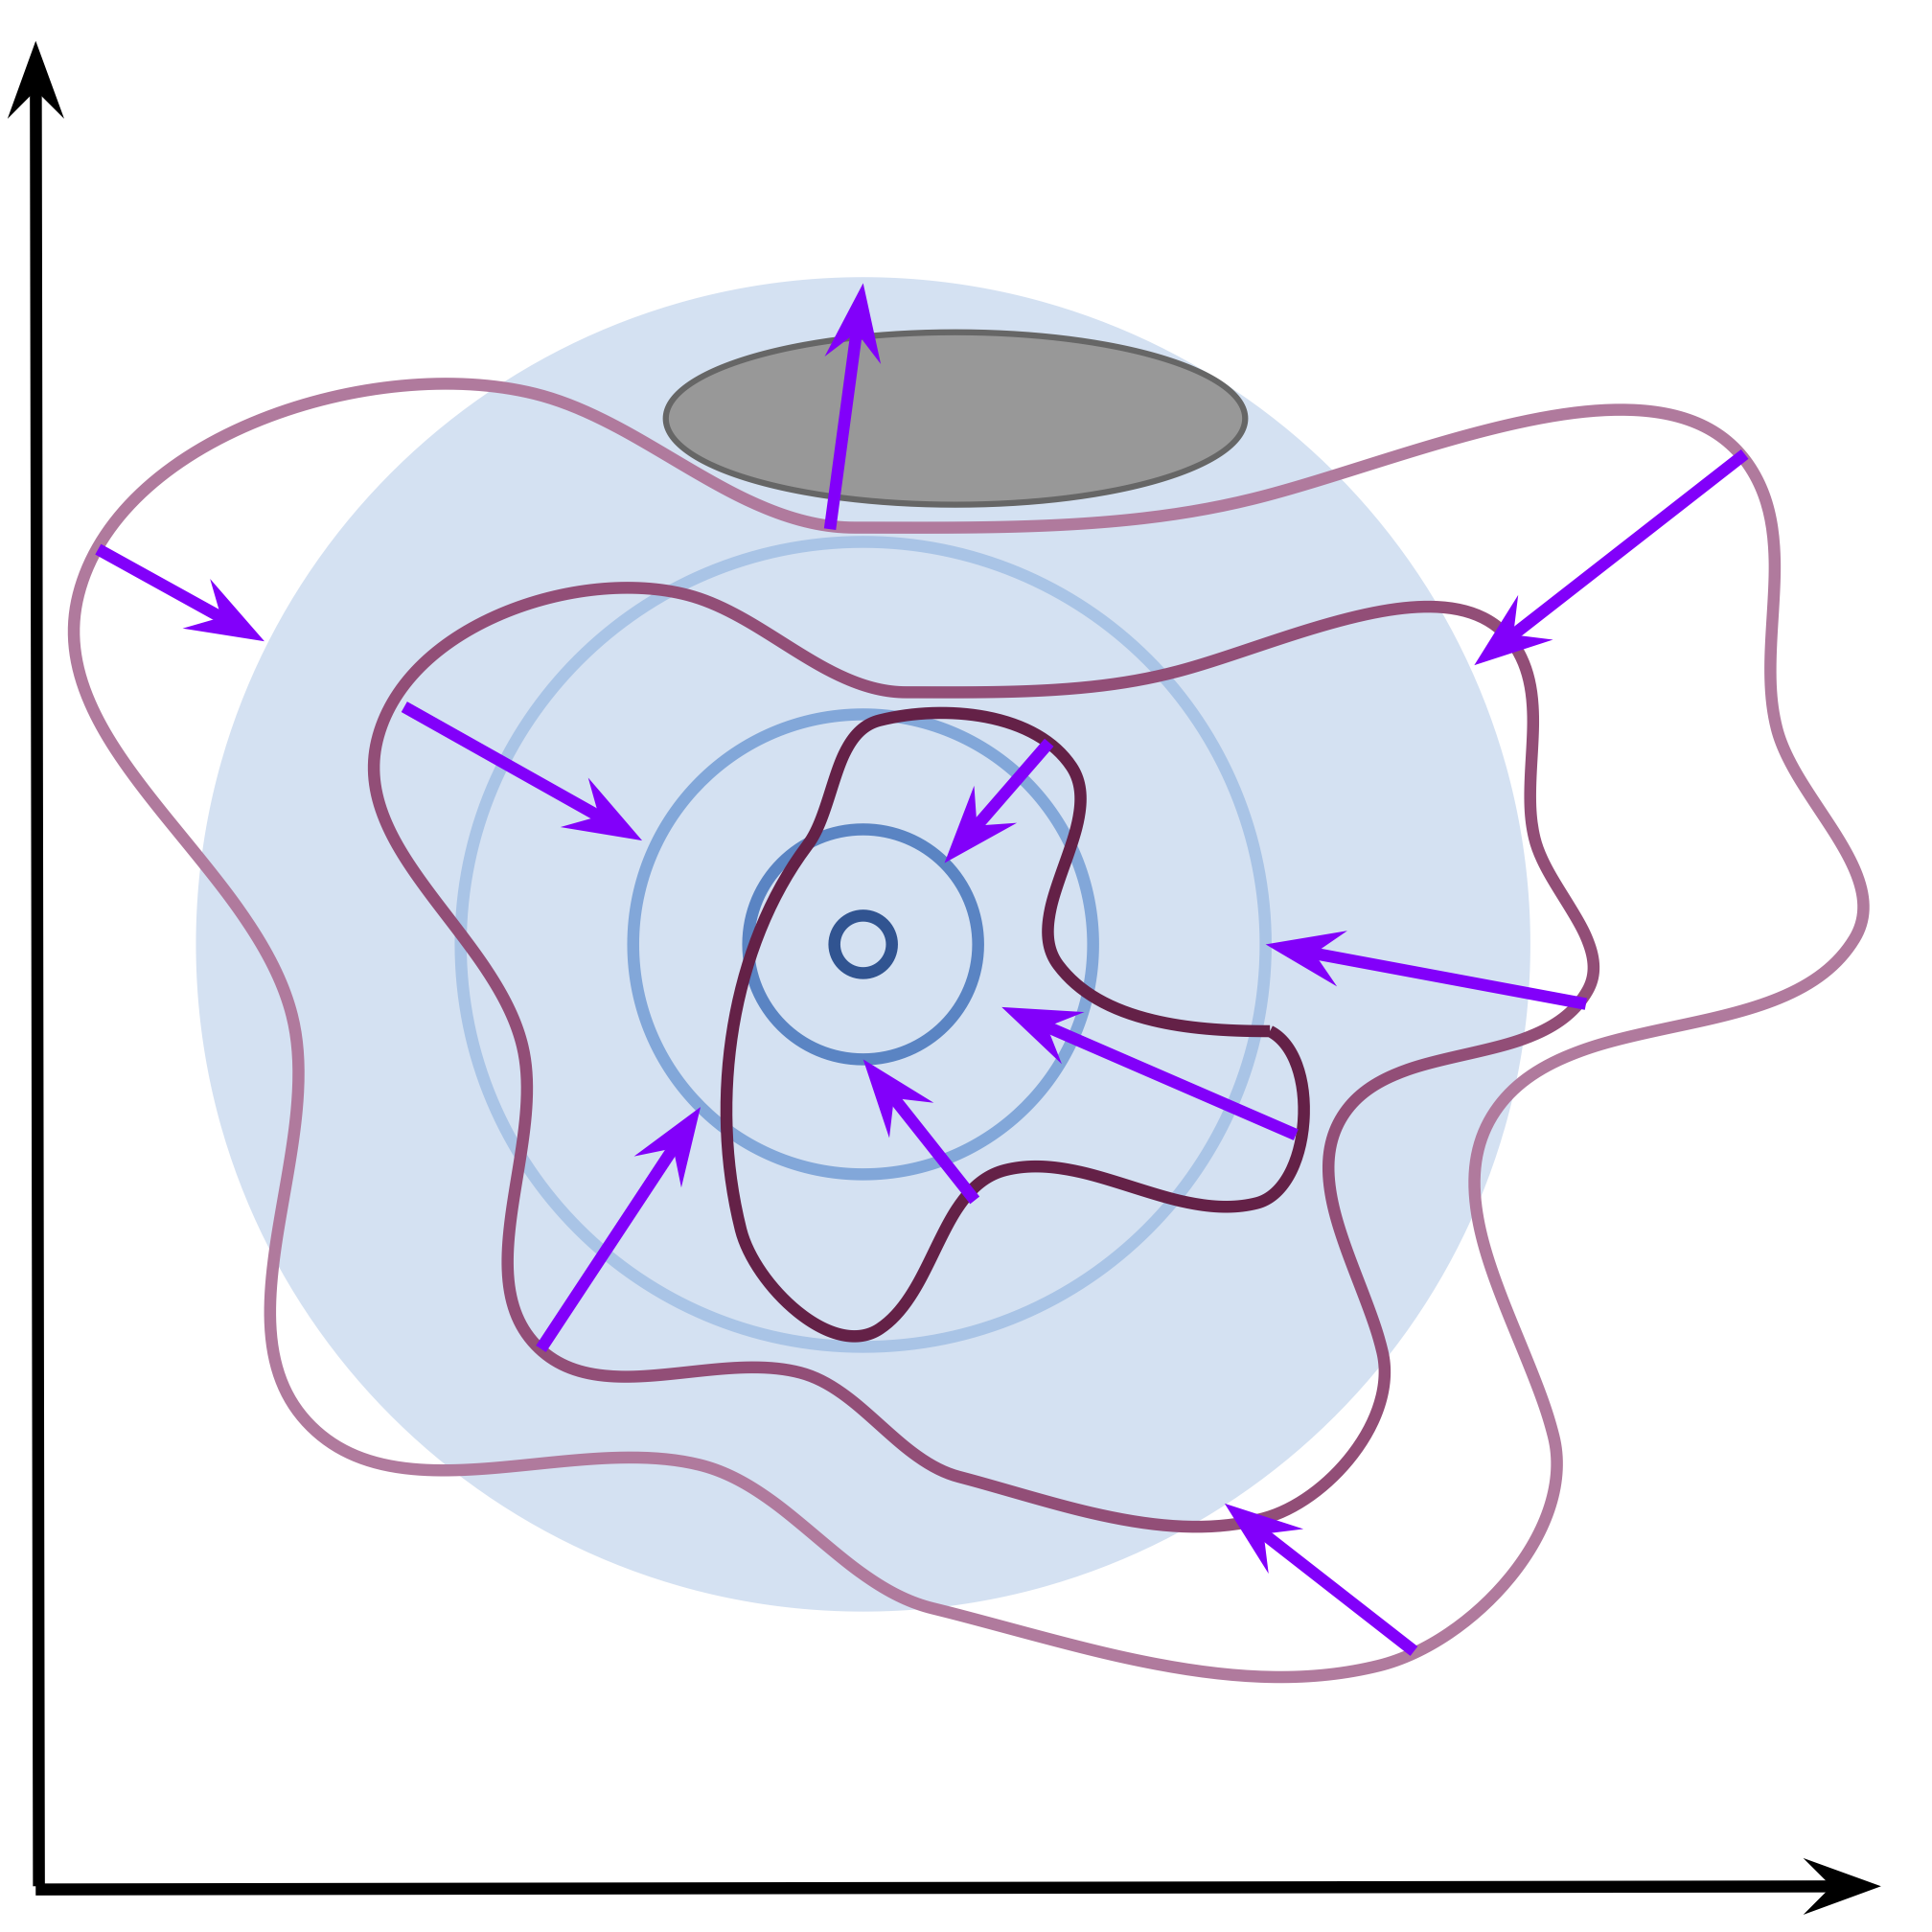
\includegraphics[width=0.8\linewidth]{figs/non_learnable_prior}
			\end{figure}
		\end{block}
	\end{minipage}%
	\begin{minipage}[t]{0.5\columnwidth}
		\begin{block}{Learnable prior $p(\bz | \blambda)$}
			\begin{figure}[h]
				\centering
				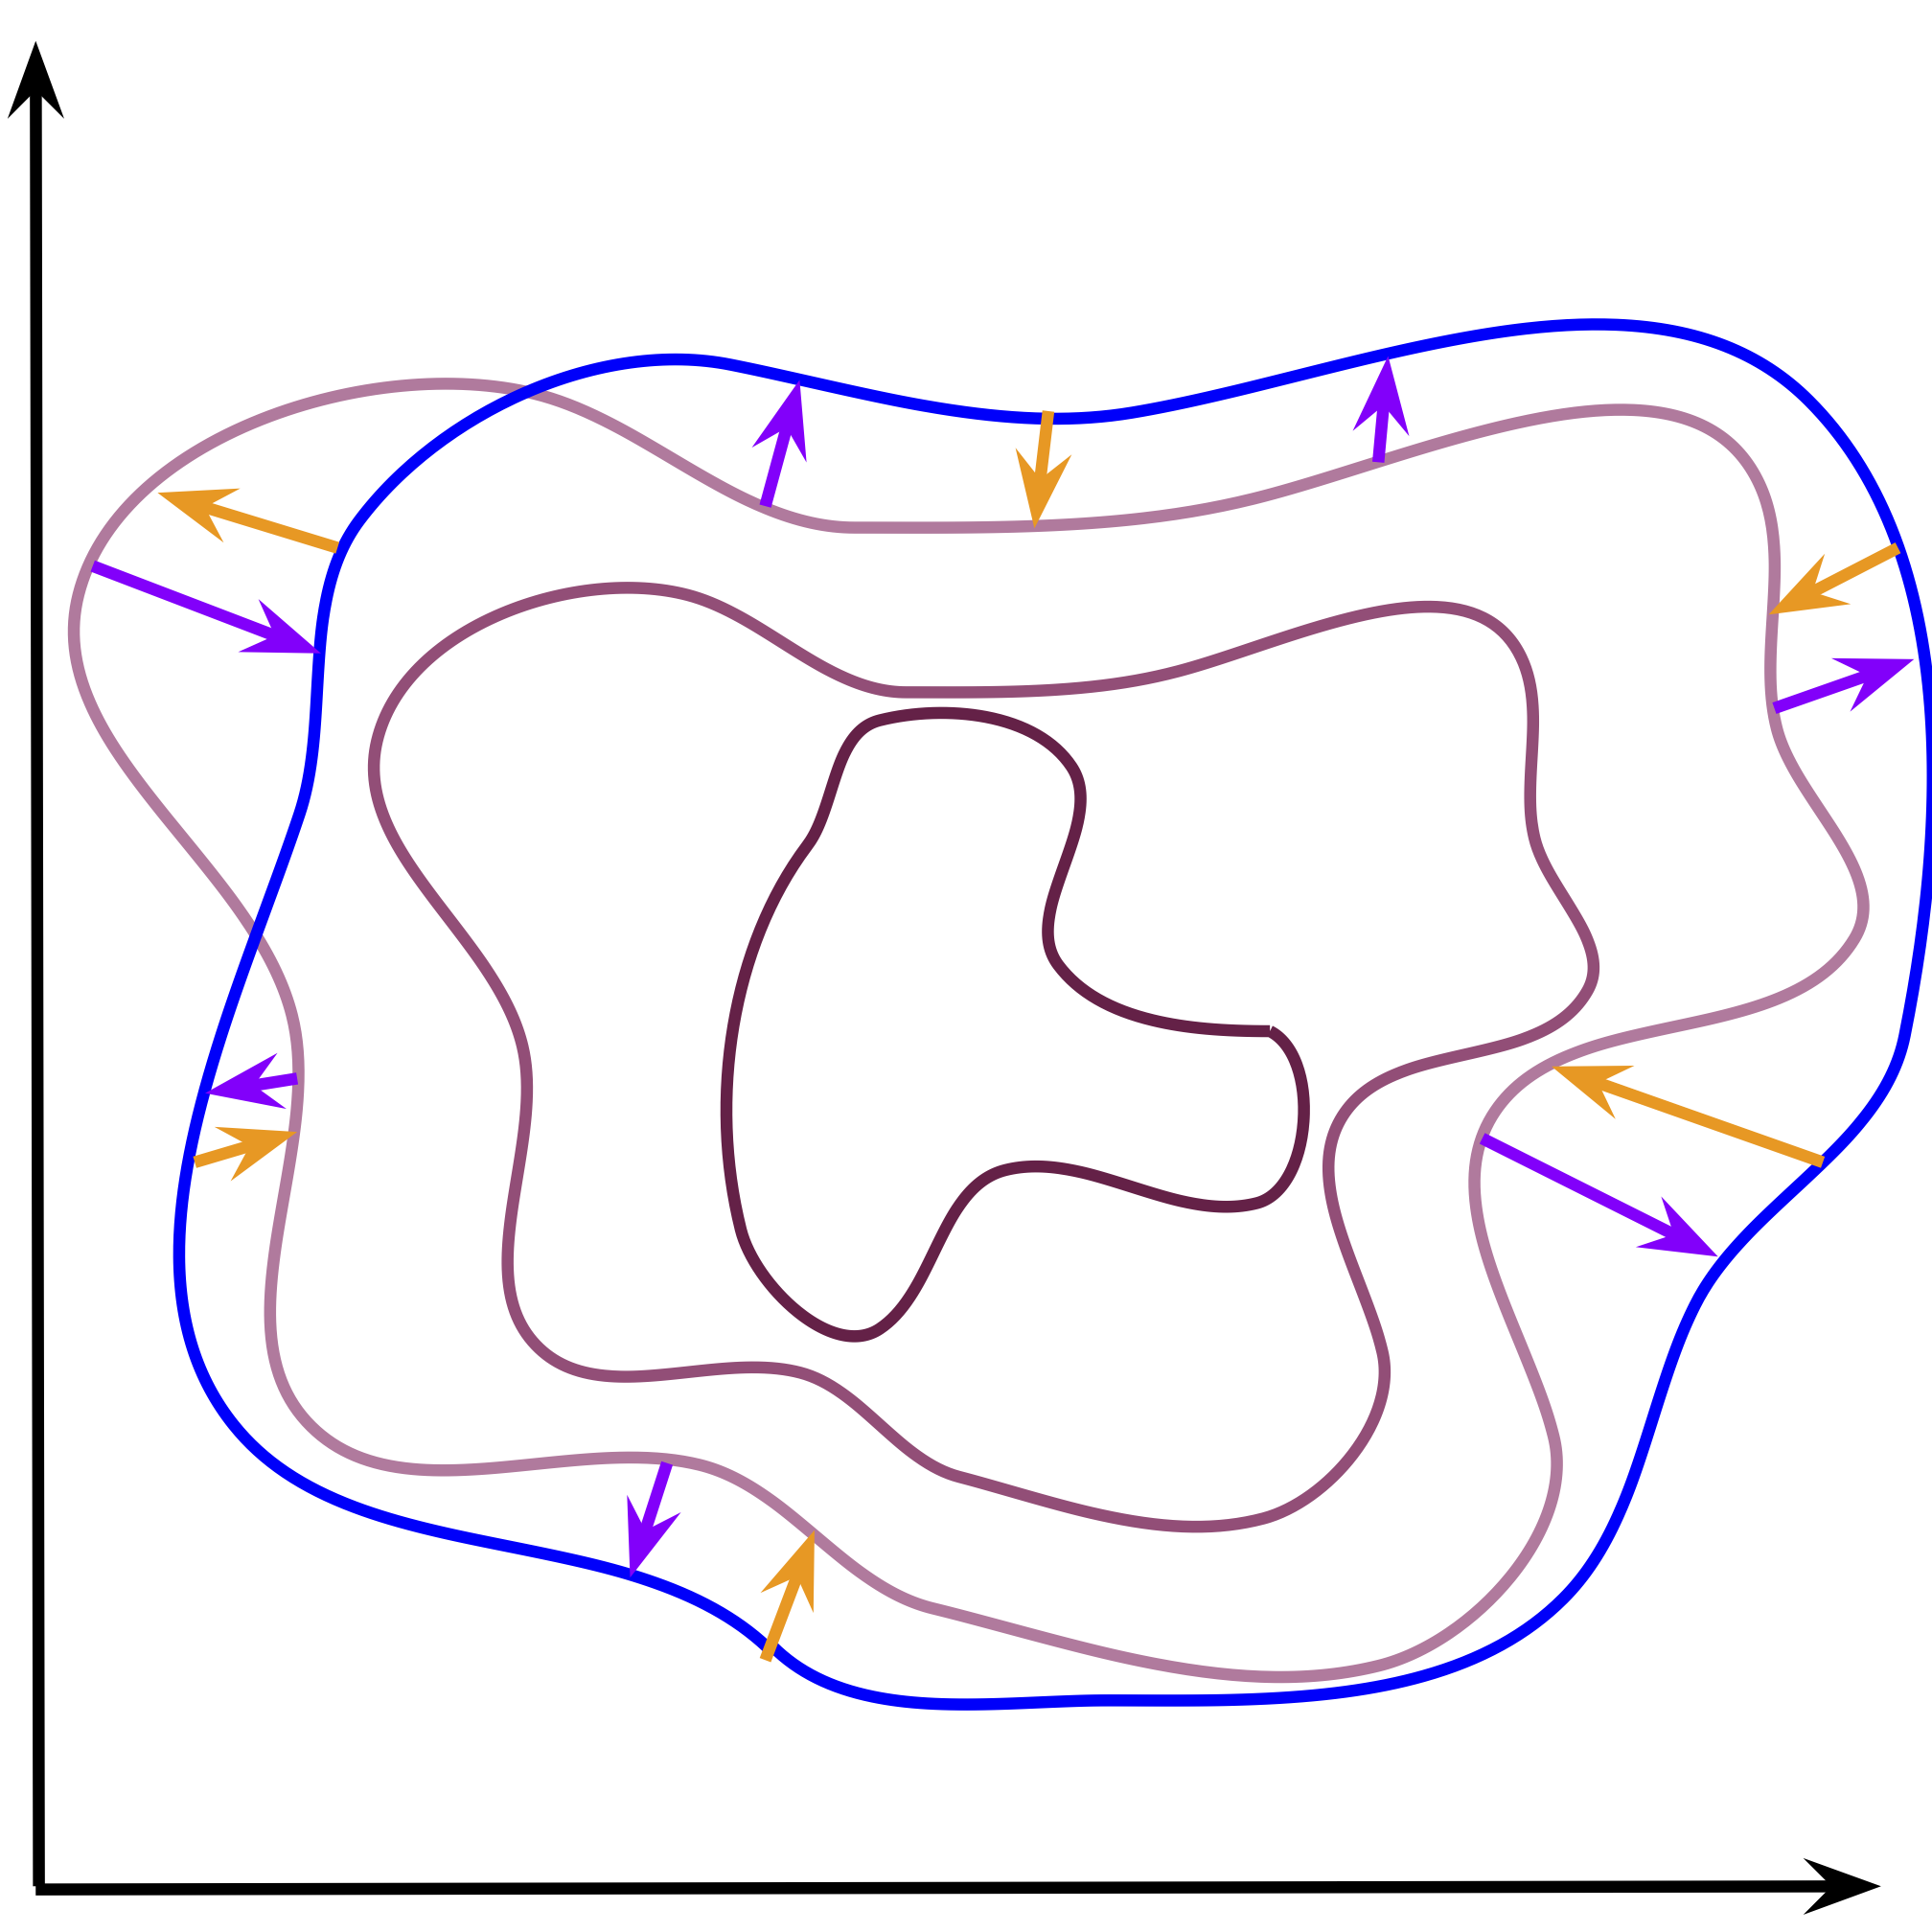
\includegraphics[width=0.8\linewidth]{figs/learnable_prior}
			\end{figure}
		\end{block}
	\end{minipage}
	\myfootnotewithlink{https://jmtomczak.github.io/blog/7/7\_priors.html}{image credit: https://jmtomczak.github.io/blog/7/7\_priors.html}
\end{frame}
%=======
\begin{frame}{Learnable VAE prior}
	\begin{block}{Optimal prior}
		\vspace{-0.7cm}
		\[
			KL(q_{\text{agg}}(\bz) || p(\bz)) = 0 \quad \Leftrightarrow \quad p (\bz) = q_{\text{agg}}(\bz) = \frac{1}{n} \sum_{i=1}^n q(\bz | \bx_i).
		\]
		\vspace{-0.6cm}
	\end{block}
	\begin{block}{Mixture of Gaussians}
		\vspace{-0.3cm}
		\[
			p(\bz | \blambda) = \sum_{k=1}^K w_k \cN(\bz | \bmu_k, \bsigma_k^2), \quad \blambda = \{w_k, \bmu_k, \bsigma_k\}_{k=1}^K.
		\]
		\vspace{-0.5cm}
	\end{block}
	\begin{block}{Variational Mixture of posteriors (VampPrior)}
		\vspace{-0.3cm}
		\[
		p(\bz | \blambda) = \frac{1}{K} \sum_{k=1}^K q(\bz | \bu_k),
		\]
		where $\blambda = \{\bu_1, \dots, \bu_K\}$ are trainable pseudo-inputs.
	\end{block}
	\begin{itemize}
		\item Multimodal $\Rightarrow$ prevents over-regularization;.
		\item $K \ll n$ $\Rightarrow$ prevents from potential overfitting + less expensive to train.
	\end{itemize}
	\myfootnotewithlink{https://arxiv.org/abs/1705.07120}{Tomczak J. M., Welling M. VAE with a VampPrior, 2017}
\end{frame}
%=======
\begin{frame}{VampPrior}
	\begin{itemize}
	\item Do we really need the multimodal prior?
	\item Is it beneficial to couple the prior with the variational posterior or the MoG prior is enough?
	\end{itemize}
	\begin{block}{Results}
		\vspace{-0.3cm}
		\begin{minipage}[t]{0.55\columnwidth}
			\begin{figure}[h]
				\centering
				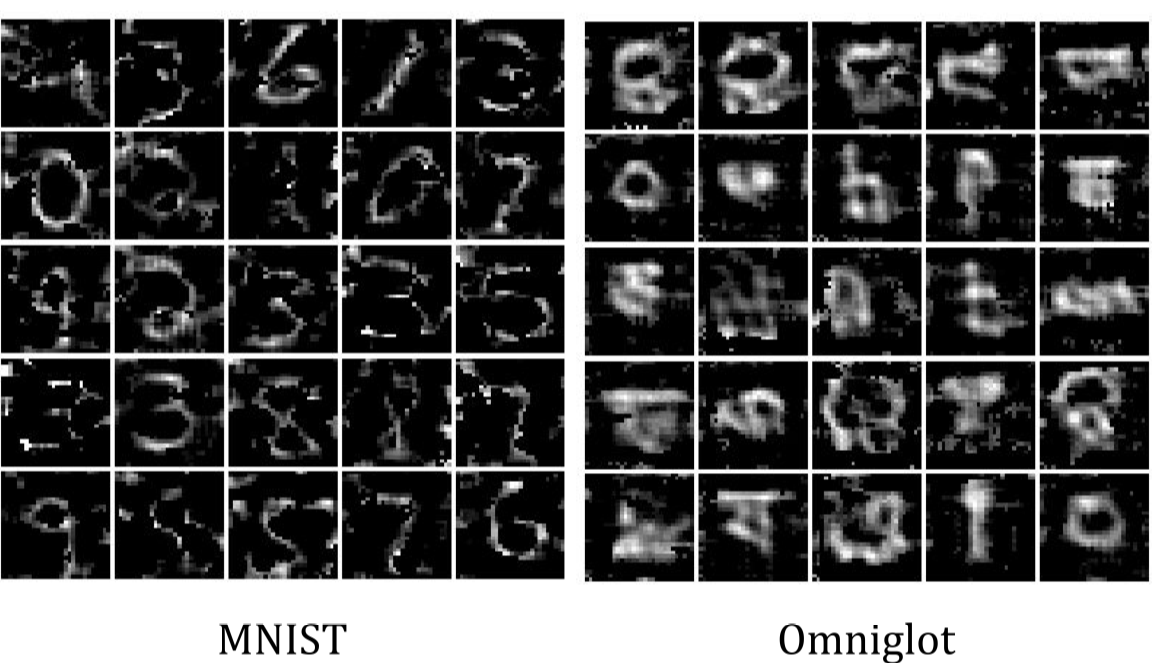
\includegraphics[width=1.0\linewidth]{figs/VampPrior_1.png}
			\end{figure}
		\end{minipage}%
		\begin{minipage}[t]{0.45\columnwidth}
			\begin{figure}[h]
				\centering
				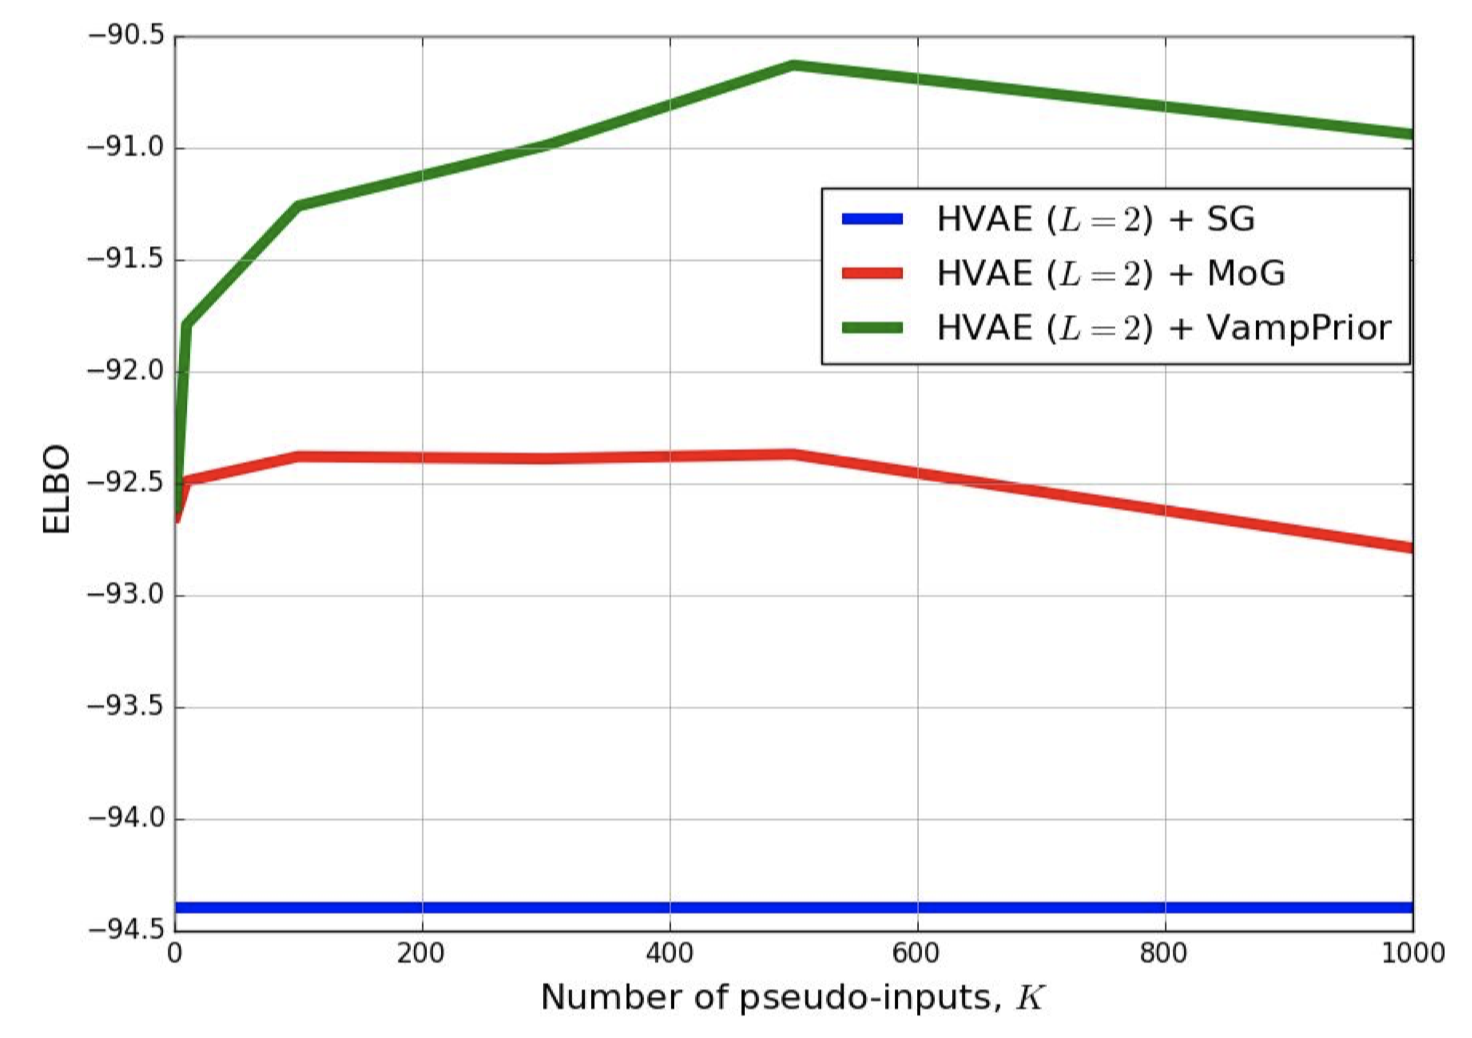
\includegraphics[width=1.0\linewidth]{figs/VampPrior_2.png}
			\end{figure}
		\end{minipage}
	\end{block}
	\textbf{Top row:} generated images by PixelHVAE + VampPrior for chosen pseudo-input in the left top corner. \\
	\vspace{0.1cm}
	\textbf{Bottom row:} pseudo-inputs for different datasets.
	\myfootnotewithlink{https://arxiv.org/abs/1705.07120}{Tomczak J. M., Welling M. VAE with a VampPrior, 2017}
\end{frame}
%=======
\begin{frame}{Flows-based VAE prior}
	\begin{block}{Flow model in latent space}
		\vspace{-0.5cm}
		\[
			\log p(\bz | \blambda) = \log p(\bepsilon) + \log \det \left | \frac{d \bepsilon}{d\bz}\right| = \log p(\bepsilon) + \log \det \left | \frac{\partial f(\bz, \blambda)}{\partial \bz}\right| 
		\]
		\[
			\bz = g(\bepsilon, \blambda) = f^{-1}(\bepsilon, \blambda)
		\]
	\end{block}
	\vspace{-0.3cm}
	\begin{itemize}
		\item RealNVP flow.
		\item Autoregressive flow (MAF).
	\end{itemize}
	Why it is not a good idea to use IAF for VAE prior?
	\begin{block}{ELBO with flow-based VAE prior}
		\vspace{-0.5cm}
		{\footnotesize
		\begin{multline*}
			\mathcal{L}(\bphi, \btheta) = \mathbb{E}_{q(\bz | \bx, \bphi)} \left[ \log p(\bx | \bz, \btheta) +  \log p(\bz | \blambda) - \log q(\bz | \bx, \bphi) \right] \\
				= \mathbb{E}_{q(\bz | \bx, \bphi)} \left[ \log p(\bx | \bz, \btheta) + \underbrace{ \Bigl( \log p(f(\bz, \blambda)) + \log \left| \det \frac{\partial f(\bz, \blambda)}{\partial \bz} \right| \Bigr) }_{\text{flow-based prior}} - \log q(\bz | \bx, \bphi) \right] 
		\end{multline*}
		}
	\end{block}
	\myfootnotewithlink{https://arxiv.org/abs/1611.02731}{Chen X. et al. Variational Lossy Autoencoder, 2016}
\end{frame}
%=======
\begin{frame}{VAE limitations}
	\begin{itemize}
		\item Poor generative distribution (decoder)
		\[
			p(\bx | \bz, \btheta) = \mathcal{N}(\bx| \bmu_{\btheta}(\bz), \bsigma^2_{\btheta}(\bz)) \quad \text{or } = \text{Softmax}(\bpi_{\btheta}(\bz)).
		\]
		\item Loose lower bound
		\[
			\log p(\bx | \btheta) - \mathcal{L}(q, \btheta) = (?).
		\]
		\item Poor prior distribution
		\[
			p(\bz) = \mathcal{N}(0, \mathbf{I}).
		\]
		\item \textbf{Poor variational posterior distribution (encoder)}
		\[
			q(\bz | \bx, \bphi) = \mathcal{N}(\bz| \bmu_{\bphi}(\bx), \bsigma^2_{\bphi}(\bx)).
		\]
	\end{itemize}
\end{frame}
%=======
\begin{frame}{Variational posterior}
	\begin{block}{ELBO}
		\[
		\log p(\bx | \btheta) = \mathcal{L}(q, \btheta) + KL(q(\bz | \bx, \bphi) || p(\bz | \bx, \btheta)).
		\]
	\end{block}
	\begin{itemize}
		\item In E-step of EM-algorithm we wish $KL(q(\bz | \bx, \bphi) || p(\bz | \bx, \btheta)) = 0$. \\
		(In this case the lower bound is tight $\log p(\bx | \btheta) = \mathcal{L}(q, \btheta)$). \\
		\item Normal variational distribution $q(\bz | \bx, \bphi) = \mathcal{N}(\bz| \bmu_{\bphi}(\bx), \bsigma^2_{\bphi}(\bx))$ is poor (e.g. has only one mode). \\
		\item Flows models convert a simple base distribution to a complex one using invertible transformation with simple Jacobian. How to use flows in VAE posterior?
	\end{itemize}
\end{frame}
%=======
\begin{frame}{Flows in VAE posterior}
	Apply a sequence of transformations to the random variable
	\[
	\bz_0 \sim q(\bz | \bx, \bphi) = \mathcal{N}(\bz| \bmu_{\bphi}(\bx), \bsigma^2_{\bphi}(\bx)).
	\]
	Let $q(\bz | \bx, \bphi)$ (VAE encoder) be a base distribution for a flow model.
	
	\begin{block}{Flow model in latent space}
		\vspace{-0.3cm}
		\[
			\log q(\bz^* | \bx, \bphi, \blambda) = \log q(\bz | \bx, \bphi) + \log \det \left | \frac{\partial f(\bz, \blambda)}{\partial \bz}\right|
		\]
		\[
			\bz^* = f(\bz, \blambda) = g^{-1}(\bz, \blambda)
		\]
	\end{block}
	Here $f(\bz, \blambda)$ is a flow model (e.g. stack of planar/coupling layers) parameterized by $\blambda$.
	
	
	Let use $q(\bz^* | \bx, \bphi, \blambda)$ as a variational distribution. Here $\bphi$~-- encoder parameters, $\blambda$~-- flow parameters.
	
	\myfootnotewithlink{https://arxiv.org/abs/1505.05770}{Rezende D. J., Mohamed S. Variational Inference with Normalizing Flows, 2015} 
\end{frame}
%=======
\begin{frame}{Flows-based VAE posterior}
	\begin{itemize}
		\item Encoder outputs base distribution $q(\bz | \bx, \bphi)$.
		\item Flow model $\bz^* = f(\bz, \blambda)$ transforms the base distribution $q(\bz | \bx, \bphi)$ to the distribution $q(\bz^* | \bx, \bphi, \blambda)$.
		\item Distribution $q(\bz^* | \bx, \bphi, \blambda)$ is used as a variational distribution for ELBO maximization.
	\end{itemize}
	
	\begin{block}{Flow model in latent space}
		\vspace{-0.3cm}
		\[
			\log q(\bz^* | \bx, \bphi, \blambda) = \log q(\bz | \bx, \bphi) + \log \det \left | \frac{\partial f(\bz, \blambda)}{\partial \bz}\right|
		\]
		\vspace{-0.3cm}
	\end{block}
	\begin{block}{ELBO with flow-based VAE posterior}
		\vspace{-0.5cm}
		\begin{align*}
			\mathcal{L} (\bphi, \btheta, \blambda)  
			&= \bbE_{q(\bz^* | \bx, \bphi, \blambda)} \bigl[\log p(\bx, \bz^* | \btheta) - \log q(\bz^*| \bx, \bphi, \blambda) \bigr] \\ 
			&=  \bbE_{q(\bz^* | \bx, \bphi, \blambda)} \log p(\bx | \bz^*, \btheta) - KL (q(\bz^* | \bx, \bphi, \blambda) || p(\bz^*)).
		\end{align*}
		\vspace{-0.4cm}
	\end{block}
	The second term in ELBO is reverse KL divergence. Planar flows was originally proposed for variational inference in VAE.
	
	\myfootnotewithlink{https://arxiv.org/abs/1505.05770}{Rezende D. J., Mohamed S. Variational Inference with Normalizing Flows, 2015} 
\end{frame}
%=======
\begin{frame}{Flows-based VAE posterior}
	
	\begin{block}{Flow model in latent space}
		\vspace{-0.3cm}
		\[
			\log q(\bz^* | \bx, \bphi, \blambda) = \log q(\bz | \bx, \bphi) + \log \det \left | \frac{\partial f(\bz, \blambda)}{\partial \bz}\right|
		\]
		\vspace{-0.3cm}
	\end{block}
	\begin{block}{ELBO objective}
		\vspace{-0.5cm}
		\begin{multline*}
			\mathcal{L} (\bphi, \btheta, \blambda)  
			= \mathbb{E}_{q(\bz^* | \bx, \bphi, \blambda)} \bigl[\log p(\bx, \bz^* | \btheta) - \log q(\bz^*| \bx, \bphi, \blambda) \bigr] = \\
			= \mathbb{E}_{q(\bz | \bx, \bphi)} \left. \bigl[\log p(\bx, \bz^* | \btheta) - \log q(\bz^*| \bx, \bphi, \blambda) \bigr]\right|_{\bz^* = f(\bz, \blambda)} = \\
			= \mathbb{E}_{q(\bz | \bx, \bphi)} \bigg[\log p(\bx, \bz^* | \btheta) -  \log q(\bz | \bx, \bphi ) + \log \left| \det \left( \frac{\partial f(\bz, \blambda)}{\partial \bz} \right) \right| \bigg].
		\end{multline*}
	\end{block}
	\begin{itemize}
		\item Obtain samples $\bz$ from the encoder $q(\bz | \bx, \bphi)$.
		\item Apply flow model $\bz^* = f(\bz, \blambda)$.
		\item Compute likelihood for $\bz^*$ using the decoder, base distribution for $\bz^*$ and the Jacobian.
	\end{itemize}
	\myfootnotewithlink{https://arxiv.org/abs/1505.05770}{Rezende D. J., Mohamed S. Variational Inference with Normalizing Flows, 2015} 
\end{frame}
%=======
\begin{frame}{Inverse autoregressive flow (IAF)}
	\vspace{-0.3cm}
	\begin{align*}
		\bx &= g(\bz, \btheta) \quad \Rightarrow \quad x_i = \tilde{\sigma}_i (\bz_{1:i-1}) \cdot z_i + \tilde{\mu}_i(\bz_{1:i-1}). \\
		\bz &= f(\bx, \btheta) \quad \Rightarrow \quad z_i = \left(x_i - \tilde{\mu}_i(\bz_{1:i-1}) \right) \cdot \frac{1}{\tilde{\sigma}_i (\bz_{1:i-1})}.
	\end{align*}
	\vspace{-0.5cm}
	\begin{block}{Reverse KL for flow model}
  		\vspace{-0.5cm}
		\[
			KL(p || \pi)  = \bbE_{p(\bz)} \left[  \log p(\bz) - \log \left|\det \left( \frac{\partial g(\bz, \btheta)}{\partial \bz} \right) \right| - \log \pi(g(\bz, \btheta)) \right]
		\]
		\vspace{-0.3cm}
	\end{block}
	\begin{itemize}
	\item We don’t need to think about computing the function $f(\bx, \btheta)$.
	\item Inverse autoregressive flow is a natural choice for using flows in VAE:
	\end{itemize}
	\vspace{-0.3cm}
	\begin{align*}
		\bz &= \bsigma(\bx) \odot \bepsilon + \bmu(\bx), \quad \bepsilon \sim \mathcal{N}(0, 1); \quad  \sim q(\bz | \bx, \bphi). \\
		\bz_k &= \tilde{\bsigma}_k(\bz_{k - 1}) \odot \bz_{k-1} + \tilde{\bmu}_k(\bz_{k - 1}), \quad k \geq 1; \quad  \sim q_k(\bz_k | \bx, \bphi, \{\blambda_j\}_{j=1}^k).
	\end{align*}
	\myfootnotewithlink{https://arxiv.org/abs/1606.04934}{Kingma D. P. et al. Improving Variational Inference with Inverse Autoregressive Flow, 2016} 
\end{frame}
%=======
\begin{frame}{Inverse autoregressive flow (IAF)}
	\begin{figure}
		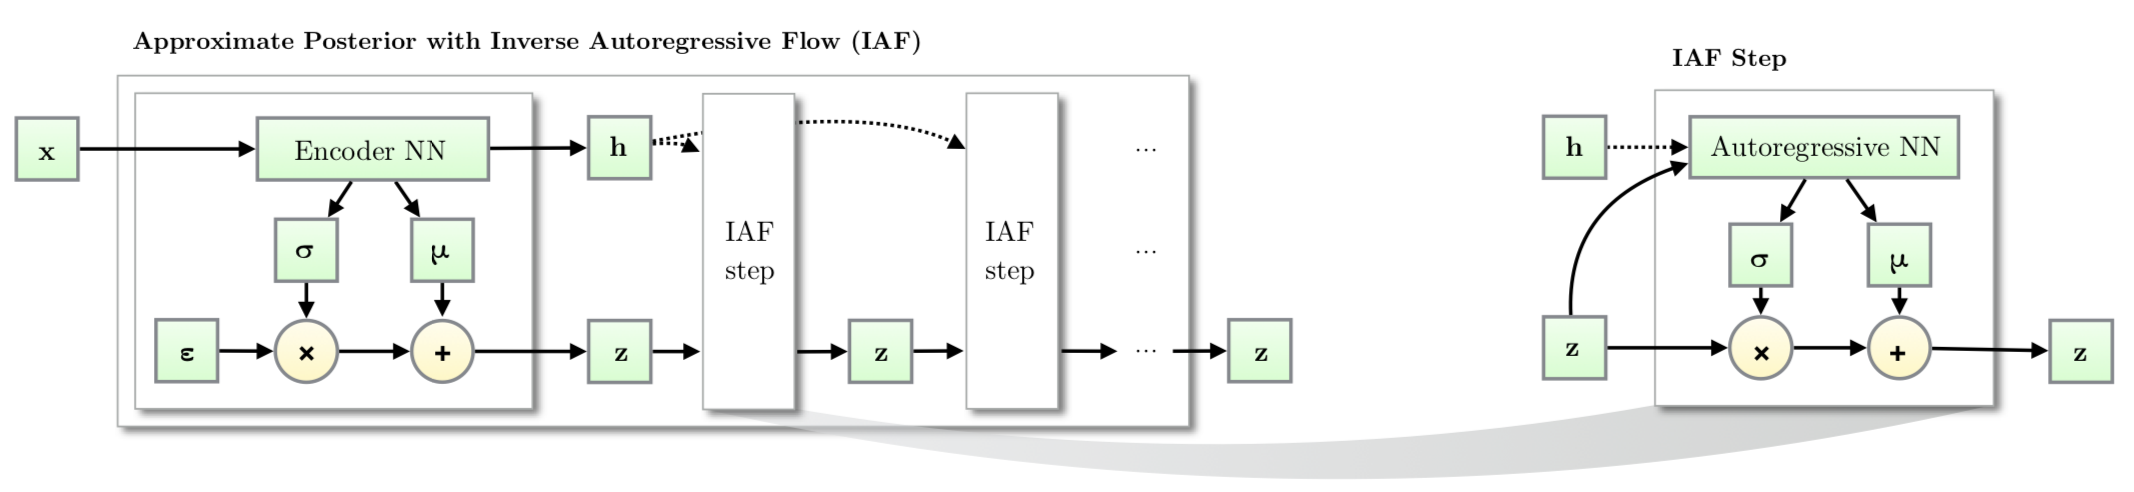
\includegraphics[width=\linewidth]{figs/iaf2.png}
	\end{figure}
	\begin{figure}
		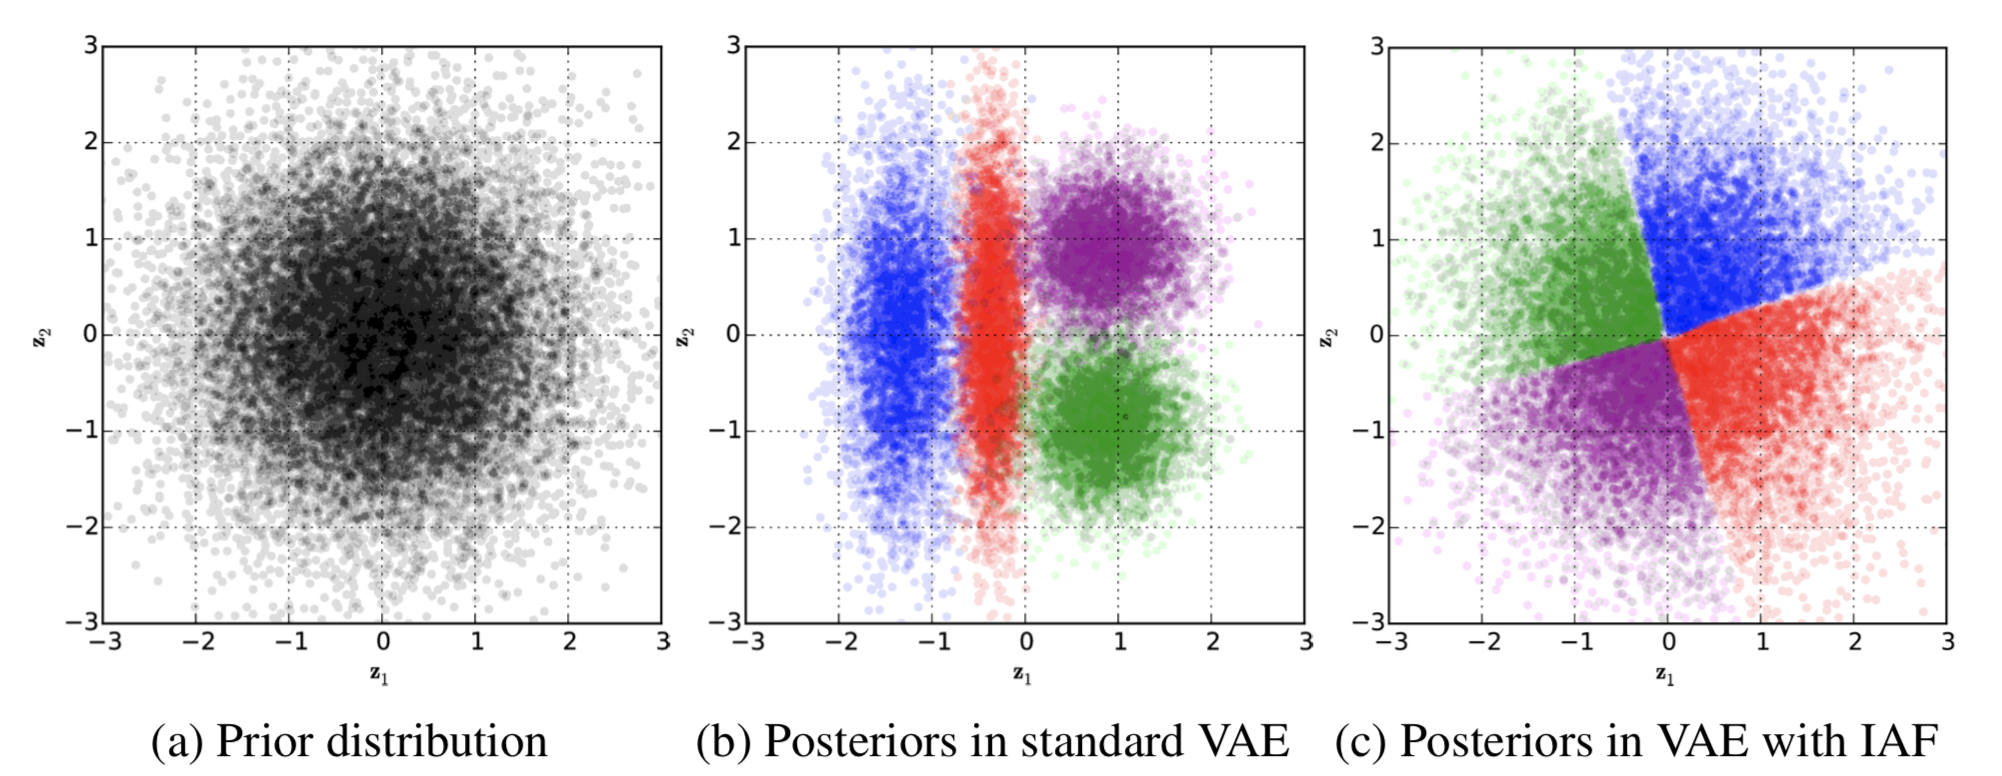
\includegraphics[width=\linewidth]{figs/iaf1.png}
	\end{figure}

	\myfootnotewithlink{https://arxiv.org/abs/1606.04934}{Kingma D. P. et al. Improving Variational Inference with Inverse Autoregressive Flow, 2016} 
\end{frame}
%=======
\begin{frame}{Flows-based VAE prior vs posterior}
	\begin{block}{Theorem}
	VAE with the flow-based prior for latent code $\bz$ is equivalent to VAE with flow-based posterior for latent code $\bz$.
	\end{block}
	\begin{block}{Proof}
	\vspace{-0.5cm}
	\begin{align*}
		\mathcal{L}(\bphi, \btheta, \blambda) &= \mathbb{E}_{q(\bz | \bx, \bphi)} \log p(\bx | \bz, \btheta) - \underbrace{KL( q(\bz | \bx, \bphi) || p(\bz | \blambda))}_{\text{flow-based prior}} \\
		& = \mathbb{E}_{q(\bz | \bx, \bphi)} \log p(\bx | \bz, \btheta) - \underbrace{KL( q(\bz | \bx, \bphi, \blambda) || p(\bz))}_{\text{flow-based posterior}}
	\end{align*}
	(Here we use Flow KL duality theorem from Lecture 4)
	\end{block}
	\begin{block}{Flows in VAE posterior}
		\vspace{-0.3cm}
		{\small
		\[
			\mathcal{L} (\bphi, \btheta, \blambda) 
			= \mathbb{E}_{q(\bz | \bx, \bphi)} \bigg[\log p(\bx, \bz^* | \btheta) -  \log q(\bz | \bx, \bphi ) +   \log \left| \det \left( \frac{\partial f(\bz, \blambda)}{\partial \bz} \right) \right| \bigg].
		\]
		}
	\end{block}
	\myfootnotewithlink{https://arxiv.org/abs/1611.02731}{Chen X. et al. Variational Lossy Autoencoder, 2016}
\end{frame}
%=======
\begin{frame}{Flows-based VAE prior vs posterior}
	\begin{itemize}
		\item IAF posterior decoder path: $p(\bx|\bz, \btheta)$, $\bz \sim p(\bz)$.
		\item AF prior decoder path: $p(\bx|\bz, \btheta)$, $\bz = g(\bepsilon, \blambda)$, $\bepsilon \sim p(\bepsilon)$. 
	\end{itemize}
	The AF prior and the IAF posterior have the same computation cost, so using the AF prior makes the model more expressive at no training time cost.

	\begin{figure}
		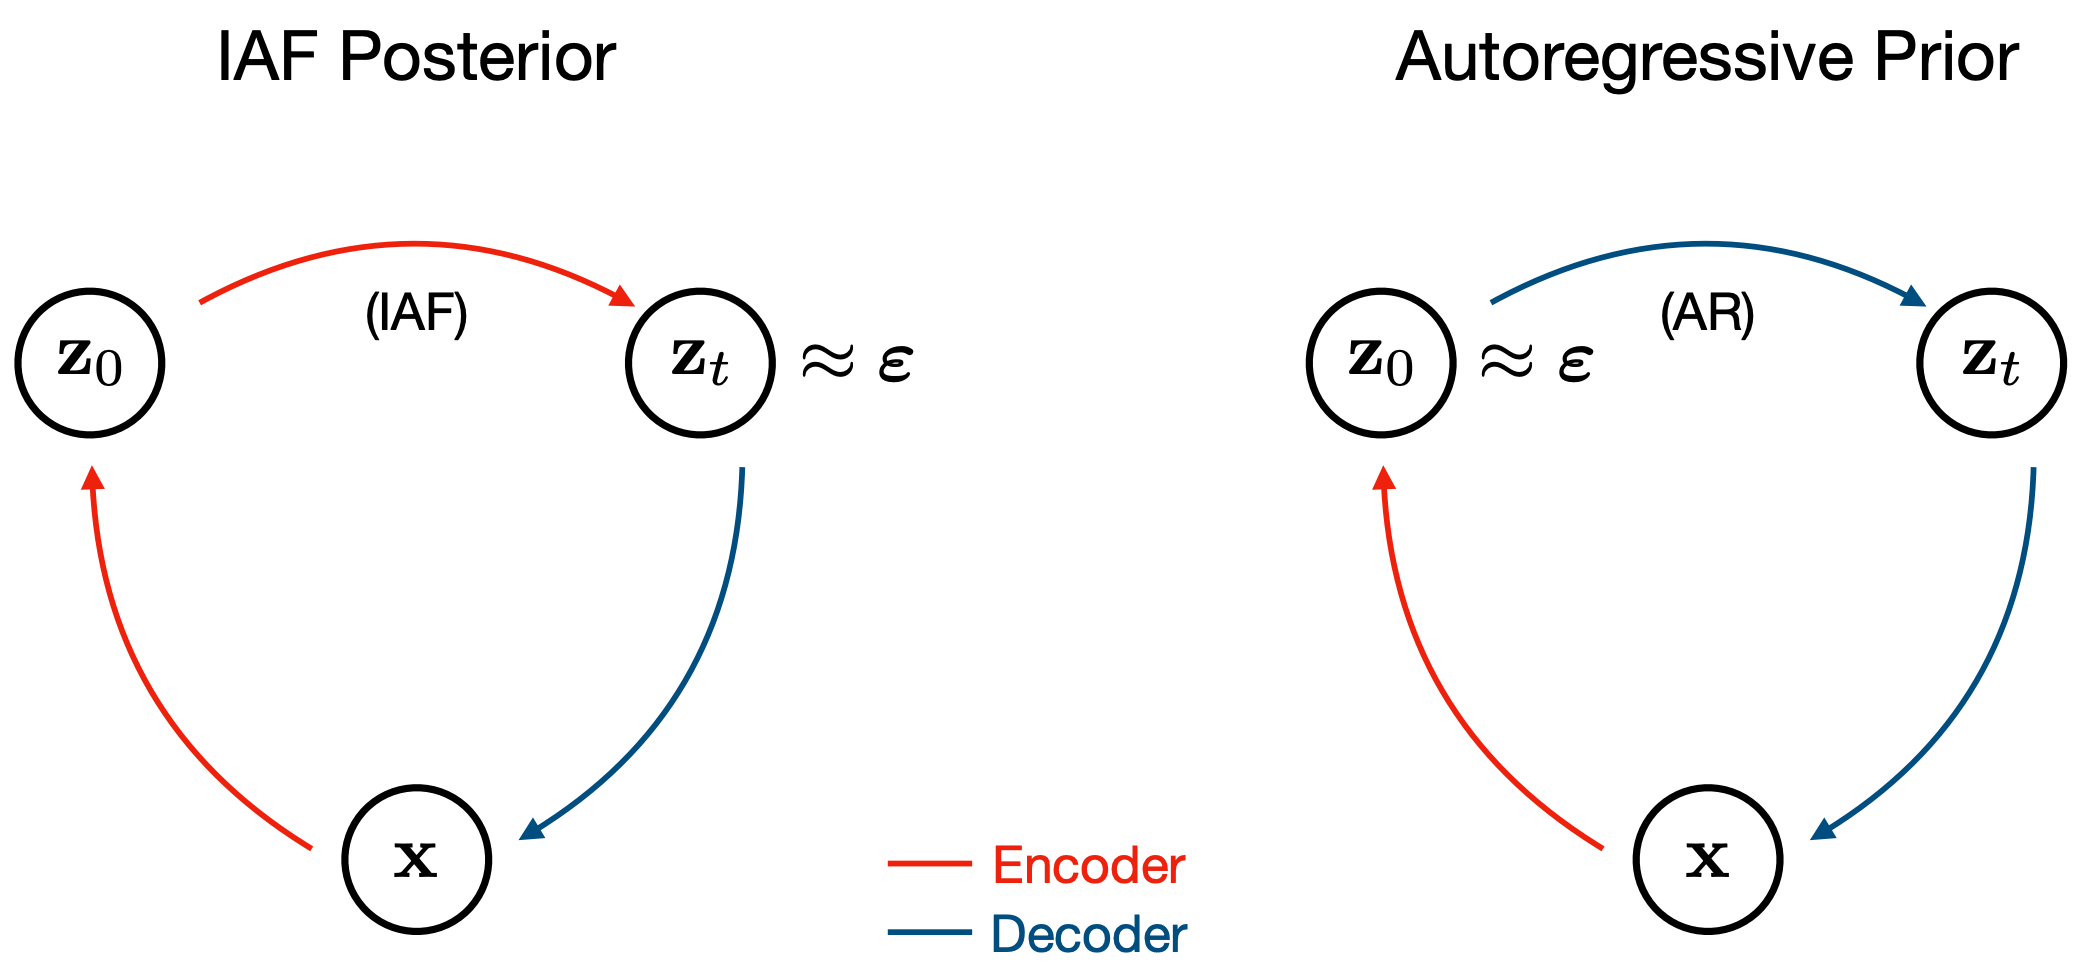
\includegraphics[width=0.85\linewidth]{figs/prior_vs_posterior}
	\end{figure}

	\myfootnotewithlink{https://courses.cs.washington.edu/courses/cse599i/20au/slides/L09_flow.pdf}{image credit: https://courses.cs.washington.edu/courses/cse599i/20au}
\end{frame}
%=======
\begin{frame}{VAE limitations}
	\begin{itemize}
		\item Poor variational posterior distribution (encoder)
		\[
			q(\bz | \bx, \bphi) = \mathcal{N}(\bz| \bmu_{\bphi}(\bx), \bsigma^2_{\bphi}(\bx)).
		\]
		\item Poor prior distribution
		\[
			p(\bz) = \mathcal{N}(0, \mathbf{I}).
		\]
		\item Poor probabilistic model (decoder)
		\[
			p(\bx | \bz, \btheta) = \mathcal{N}(\bx| \bmu_{\btheta}(\bz), \bsigma^2_{\btheta}(\bz)).
		\]
		\item Loose lower bound
		\[
			\log p(\bx | \btheta) - \mathcal{L}(q, \btheta) = (?).
		\]
	\end{itemize}
\end{frame}
%=======
\begin{frame}{Summary}
	\begin{itemize}
		\item The ELBO surgery reveals insights about a prior distribution in VAE. The optimal prior is the aggregated posterior.
		\vfill
		\item VampPrior proposes to use a variational mixture of posteriors as the prior to approximate the aggregated posterior.
		\vfill
		\item We could use flow-based prior in VAE (moreover, autoregressive).
		\vfill
		\item We could use flows to make variational posterior more expressive. This is equivalent to the flow-based prior. 
	\end{itemize}
\end{frame}

\end{document} 